\documentclass[conference,a4paper,xcolor=table]{IEEEtran}


%% Language and font encodings
\usepackage[english]{babel}
\usepackage[utf8x]{inputenc}
\usepackage[T1]{fontenc}
\usepackage{cite}

%% Useful packages
\usepackage{amsmath}
\usepackage{graphicx}
\usepackage[colorinlistoftodos]{todonotes}
\usepackage[resetlabels,labeled]{multibib}
\usepackage{todonotes}
\usepackage{multirow}

% Packages for building tables and tabulars 
\usepackage{array}
\usepackage{tabu}   % Wide lines in tables
\usepackage{xspace} % Non-eatable spaces in macros

% Including graphical images and setting the figure directory
 

%% Misc Packages
\usepackage{lipsum}  
\usepackage{subcaption}

\begin{document}

\title{Coverage Analysis of NB-IoT and Sigfox: \par Two Estonian University Campuses as a Case Study}

\author{Nishant Poddar\textsuperscript{*}, Sikandar Zulqarnain Khan\textsuperscript{**}, Jakob Mass\textsuperscript{*}, Satish Narayana Srirama\textsuperscript{*}  \\
\textsuperscript{*}University of Tartu, Institute of Computer Science, Tartu, Estonia\\
\textsuperscript{**}Thomas Johann Seebeck Department of Electronics, Tallinn University of Technology, Tallinn, Estonia\\
poddar@ut.ee, sikandar.khan@taltech.ee, jakob.mass@ut.ee, \\ satish.srirama@ut.ee}

\maketitle

\begin{abstract}
Low Power Wide Area Networks (LPWANs) have become an important technology for the Internet of Things, as they provide radio coverage in the order of kilometers and enable battery-powered devices to operate for years.
This paper presents the results of an in-field investigation of the coverage analysis of two LPWAN technologies i.e., NB-IoT and Sigfox, conducted on university campuses in the two main cities of Estonia, i.e. Tartu and Tallinn.  The experiments consider two commercially available NB-IoT operators and the single Sigfox operator in Estonia. 
Most of the existing literature on NB-IoT coverage is replete with RSSI-based coverage analyses. However, RSSI is most of the time not sufficient for evaluating LTE-based technologies including NB-IoT. Thus, our investigation of NB-IoT coverage considers three parameters: RSSI, RSRP, and RSRQ such that in situations where RSSI values are unavailable, the coverage analysis is based on RSRP and RSRQ. For Sigfox coverage, we base our analysis only on the RSSI factor as for a Sigfox network the RSSI is rarely lost. Both technologies are evaluated in indoor, outdoor and deep-indoor/underground environments so as to provide an understanding of their coverage in various propagation and penetration conditions. Our results indicate that in outdoor scenarios, both Sigfox and NB-IoT achieve good to excellent coverage with almost 0\% packet losses. However, in indoor scenarios, few packet losses were observed in Sigfox while no packet losses were observed in NB-IoT, even with a weaker coverage, and possibly due to re-transmissions that is a salient feature of the NB-IoT making it more reliable than its competitive LPWAN technologies. However, in deep-indoor or underground scenarios, coverage outages were recorded for NB-IoT, especially in Tartu area, indicating its weaker coverage in that city.
\end{abstract}

\begin{IEEEkeywords}
LPWAN, NB-IoT, Sigfox, LoRaWAN, coverage, network-testing, RSRP 
\end{IEEEkeywords}

\section{INTRODUCTION}
Low Power Wide Area Networks (LPWANs) provide long range transmissions allowing for a communication range of up to 40 km in rural zones and up to 10 km in urban zones\cite{centenaro2016long}, low development cost with device price as low as \$5, low energy profiles with battery life of up to 10 years or more\cite{patel2017experimental}, and low operator subscription costs\cite{raza2017low}. The basic motivation behind LPWAN technologies is transmitting a few short-length messages per day or weeks and even months in the long and mid radio range for supporting Internet of Things (IoT) applications. It is for these various reasons that many LPWAN technologies have been introduced, both in the licensed and unlicensed frequency spectra, to fulfil the various needs of diverse IoT applications. Among the available LPWAN technologies, Sigfox, LoRaWAN, and NB-IoT are the most prevalent and emerging technologies, with technical differences though, that are selected as per the individual application requirements \cite{mekki2018overview}.\par
Sigfox technology was developed by a French start-up in 2010 and has ever since attracted a great deal of interest from the industry, academia and standards developing organizations. Sigfox provides promising results in terms of long range, low power and low cost and has been deployed in more than 70 countries around the globe \cite{sigfoxCoverage}. A typical Sigfox device that is powered by a 2400 mAh battery can achieve a theoretical lifetime of 2.5 years while sending one message every 10 min at 100 or 600 bits/s depending on the region, and an asymptotic lifetime of 14.6 years if the message transmission rate decreases \cite{gomez2019sigfox}.\par
LoRaWAN was developed by another French start-up named Cycleo in 2009 and was later purchased by Semtech (USA) in 2012. In 2015, LoRaWAN was standardized by the LoRa-Alliance and is currently deployed across 42 countries. It is still under roll-out in many countries due to the interests of various mobile operators, industrial partners and academic researchers. As per the current specification it supports data rate up to 50 kbps in both uplink and downlink, depending on the spreading factors \cite{mekki2018overview}. \par
NB-IoT allows long-range communications at low data rates and is most suitable for delay-tolerant applications. It can provide a data rate of 250 kbps for multi-tone downlink communication and 20 kbps for single-tone uplink communications. For data collection at the lowest layer, NB-IoT utilizes end-nodes that are powered by
chargeable batteries and are embedded with sensors for gathering data from their surroundings. The device complexity of NB-IoT nodes is reduced as compared to other unlicensed LPWAN technologies, including LTE-Cat M1 devices, for addressing the ultralow-power IoT applications. The NB-IoT nodes feature battery saving modes such as PSM and eDRX to achieve higher energy efficiency and longer battery life where the future NB-IoT nodes are expected to have a battery life of more than 10 years as per the standard.

\subsection{Motivation and Related Work}
Although many efforts have been put to compare the various performance parameters of the available LPWAN technologies, they are limited in the sense that most of the conclusions are based on very few or restricted number of parameters. For example, the authors in \cite{malik2019nb} produced empirical results for NB-IoT network trial, but their conclusions were based on only one performance indicator i.e., RSSI. Based on their one-factor conclusions they claimed that NB-IoT provides good connectivity in an indoor and outdoor scenario but do not provide any good performance in deep-indoor/underground scenarios. The same authors in \cite{khan2019dorm} claimed good performance of NB-IoT coverage in an indoor scenario at different elevation levels, but their conclusions were based on only two factors i.e. RSSI and SNR. Similarly, the authors in \cite{lauridsen2017coverage} produced simulation-based coverage analysis of GPRS, Sigfox, LoRa and NB-IoT for indoor and outdoor scenarios but provided no details on how these simulation-based results could be related to real-world scenarios. However, the same authors in their work \cite{vejlgaard2017coverage} compared the coverage and capacity analysis of SigFox, LoRa, GPRS, and NB-IoT  using a real site deployment covering 8000 km\textsuperscript{2} in Northern Denmark. Similarly, the authors in \cite{mekki2018overview} made a comprehensive overview of the LPWAN technologies and concluded that Sigfox achieves highest network coverage among all the available LPWAN technologies.\par

\begin{figure}[hb!]
\centering
    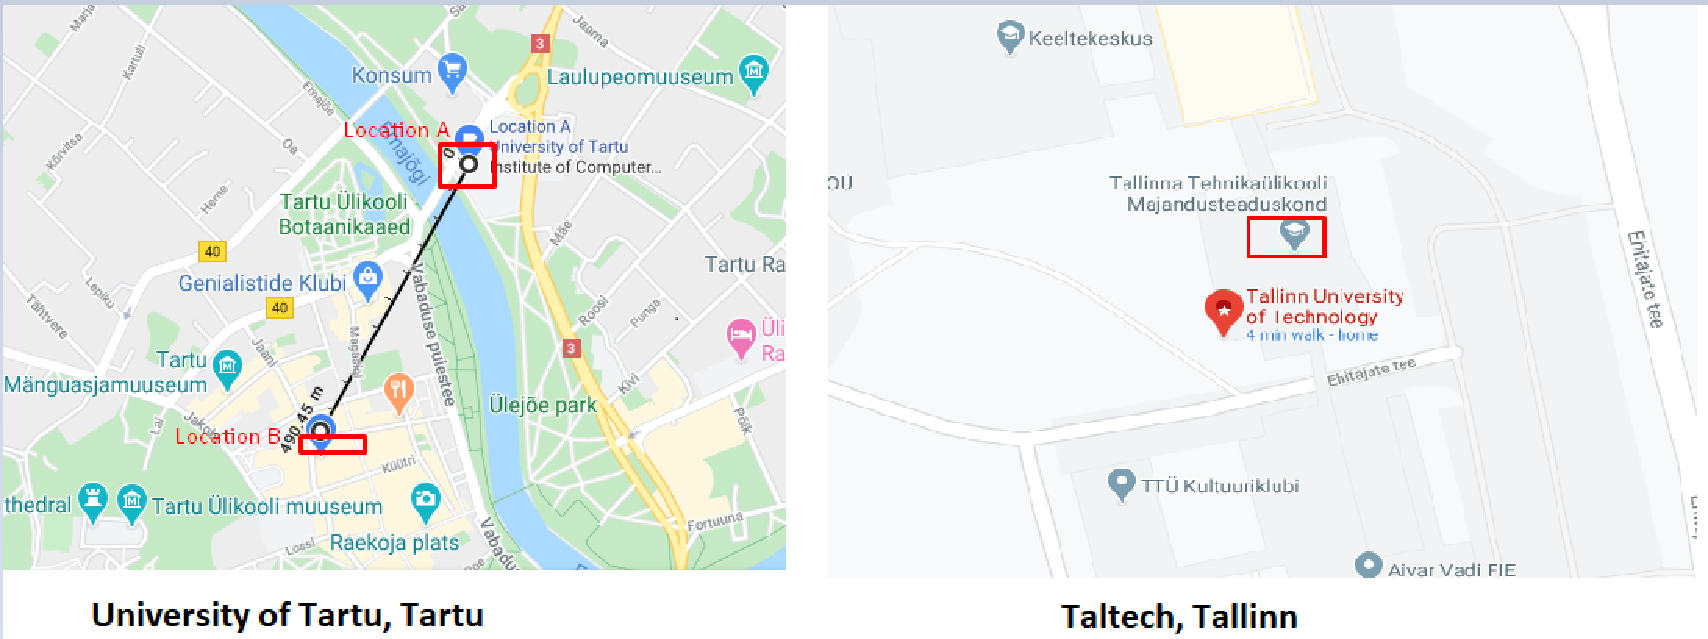
\includegraphics[width=\columnwidth]{images/locations.pdf}
    \caption{Location of measuring points in Tartu (Location A and Location B at University of Tartu, left) and Tallinn (TalTech, right)}
    \label{campus}
\end{figure}


In this work, we propose to advance the understanding of choosing among the available LPWAN operators based on their network performance (connectivity), reliability, scalability, and provided services within two Estonian cities (Tartu and Tallinn) as a use case. Our goal is to give a comparison of the LPWAN technologies in Tartu and Tallinn university campuses, however, due to limited availability of LoRaWAN network it has been excluded, and we focus on analysing the coverage performance of NB-IoT and Sigfox only. Furthermore, we consider only the uplink data for our analysis. The locations chosen for our observations include \textit{Delta} and \textit{Paabel} buildings located at the University of Tartu (UT), and Thomas Johann Seebeck Department of Electronics located at Tallinn University of Technology (TalTech), as shown on the maps in Figure \ref{campus}. We base our conclusions on three parameters analysis i.e., RSSI, RSRP, and RSRQ where RSRP and RSRQ are important indicators to be considered for analysing the LTE technologies\cite{afroz2015sinr,basu2019experimental}.\par
The remainder of the paper is organized as follows. Section \ref{Overview of NB-IoT and Sigfox} presents the overview of the current LPWAN technologies that are publicly available in Estonia. Section \ref{experimental setup} presents our experimental setup providing details of the NB-IoT and Sigfox nodes that were deployed at the above mentioned locations for data collection. Analysis and results are provided in Section \ref{results}. Section \ref{conclusion} concludes this work with future directions.

\section{Overview of the publicly available LPWAN technologies across Estonia}\label{Overview of NB-IoT and Sigfox}

There are four main public LPWAN service providers in Estonia i.e. Telia Eesti AS, Elisa Eesti AS, Connected Baltics OÜ, and Levikom Eesti OÜ; each providing a different LPWAN technology across Estonia. Telia and Elisa operate the NB-IoT technology and cover around 90\% of the whole territory of Estonia by providing service to the entire population of Estonia. This covered geography is indicated by the large shaded ellipsoid in Figure \ref{CoverageEstonia}. Connected Baltics is the exclusive Sigfox operator in Estonia and covers the major cities of Estonia: Tallinn, Tartu, Pärnu and Narva by covering around 70\% of the Estonian population \cite{connected}. The geographic coverage of Sigfox across the major cities of Estonia from the Connected Baltics is indicated by small heated circles (red, blue and green) as shown in Figure \ref{CoverageEstonia} (\cite{connected}). LEVIKOM \cite{levikom} provides LoRaWAN services but no details about their coverage in Estonia and thus we have omitted showing their coverage in Figure \ref{CoverageEstonia}. \par 


\begin{figure}[h!]
\centering
    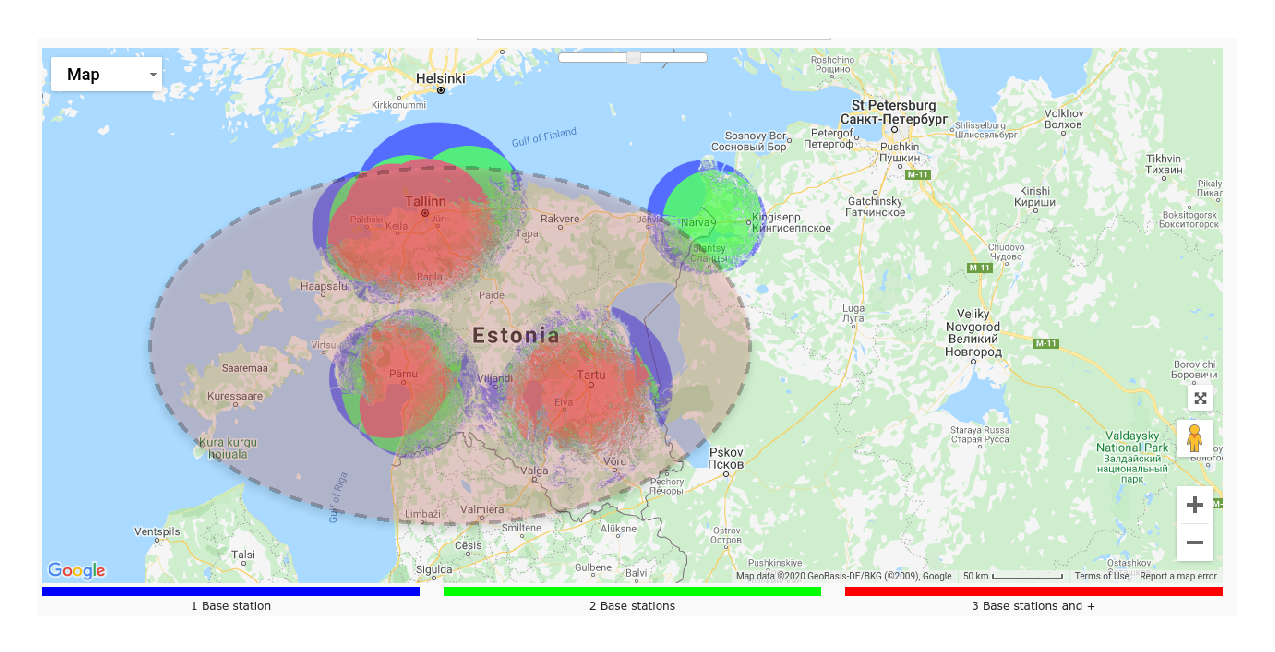
\includegraphics[width=0.8\columnwidth]{images/coverage.pdf}
    \caption{Sigfox (red, blue, green smaller circles) and NB-IoT (large shaded ellipsoid) coverage in Estonia}
    \label{CoverageEstonia}
\end{figure}


\section{Experimental Setup}\label{experimental setup}
To measure the RF values, we have used the below hard-wares in shorter time-span (half-day/day) and single cloud platform Ubidots \cite{ubidots} for data collection and analysis.
\subsection{NB-IoT Node}
We used NB-IoT DORM nodes \cite{khan2019dorm} for deployment and data collection; these devices were deployed at various locations inside and outside the main buildings of the two campuses at TalTech and University of Tartu to cover up the area. These devices were inserted with NB-IoT SIM cards from the two different NB-IoT operators (referred to as Operator A and Operator B in the rest of this paper). The DORM nodes were programmed to transmit data packets every 30 minutes. These included RSSI, RSRP, and RSRQ  values. The transmitted data packets were received and collected at a freely-available cloud platform i.e., Ubidots\cite{ubidots} for further analysis and investigation.
\begin{figure}[h!]
\centering
    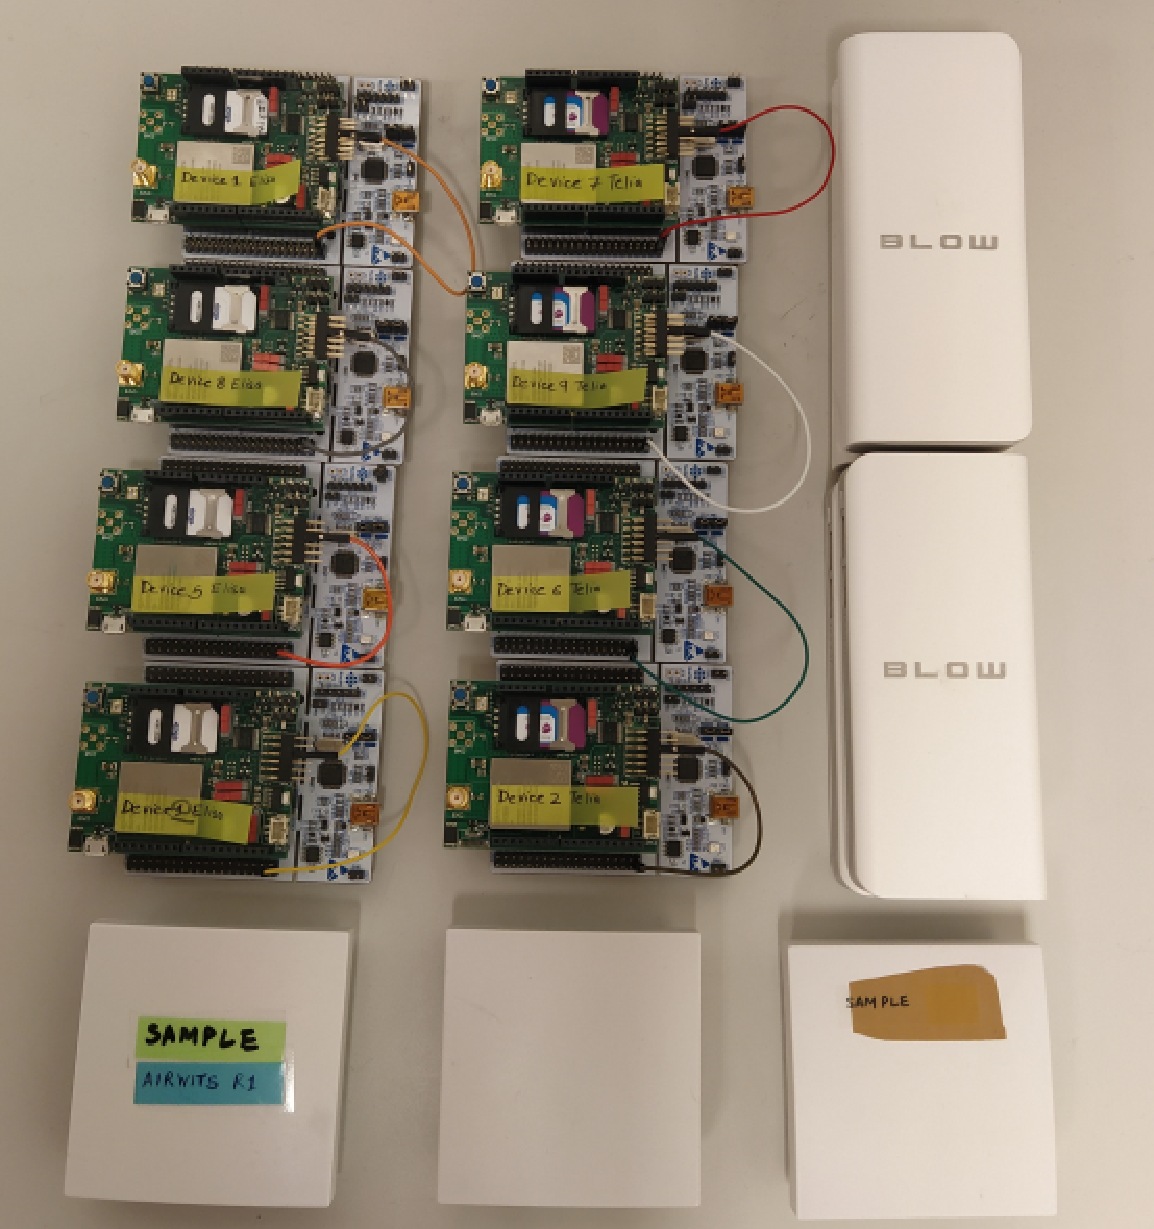
\includegraphics[width=0.8\columnwidth,height=6cm, keepaspectratio]{images/deployment images/experiment setup.pdf}
    \caption{Some of the NB-IoT (uncased) and Sigfox nodes, and batteries}
    \label{devices}
\end{figure}

 % deployment figure
\begin{figure}[h]
\centering
\begin{subfigure}[t]{0.3\linewidth}
  \centering
  % include first image
  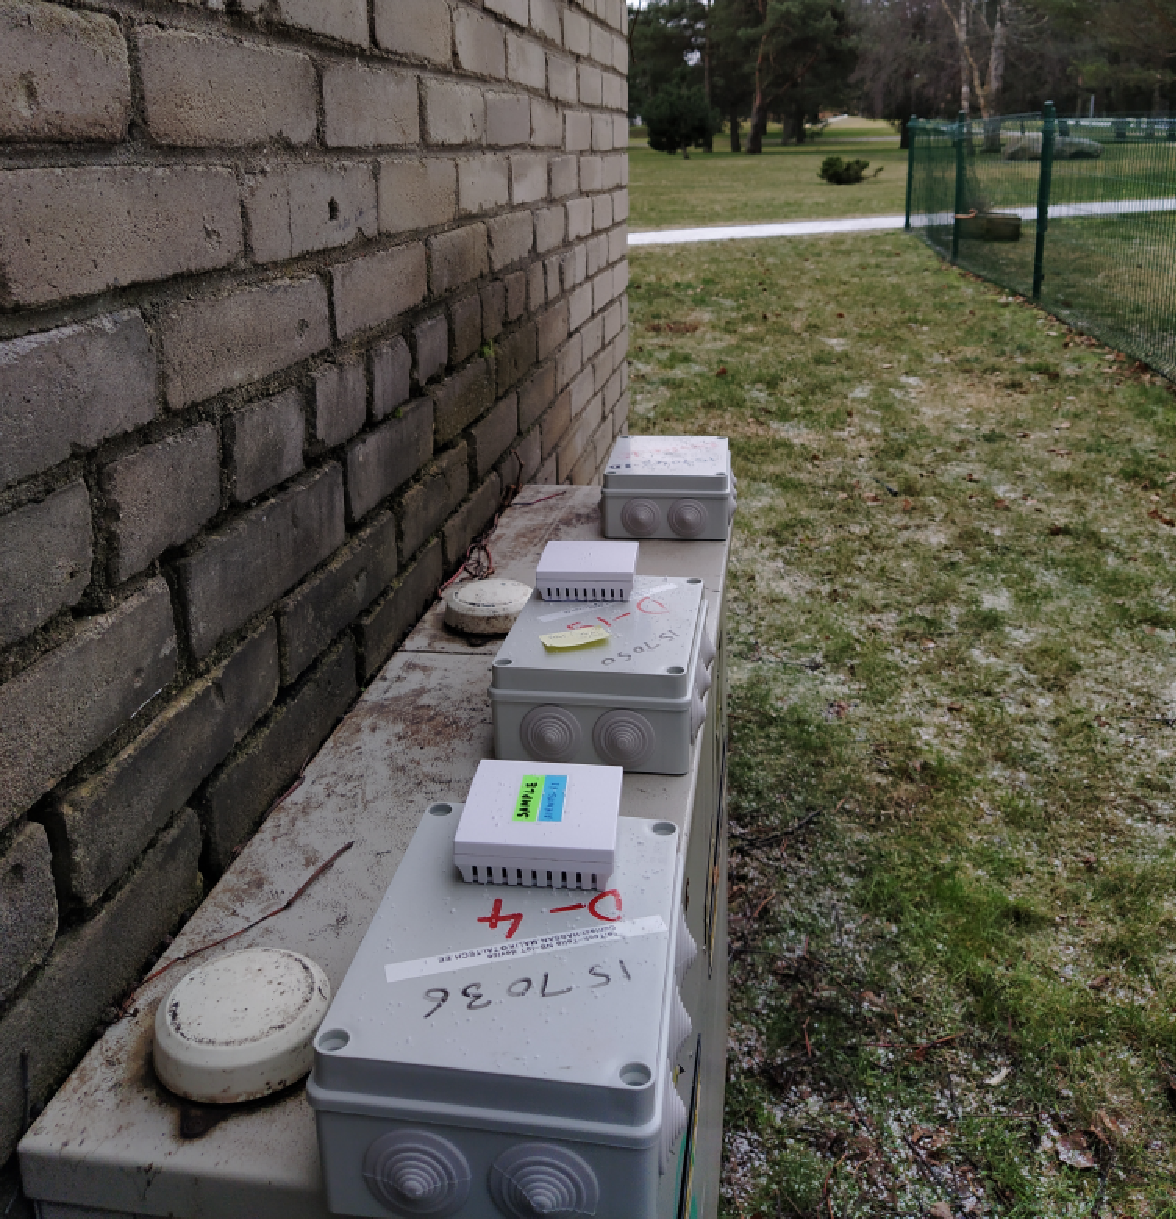
\includegraphics[width=\linewidth,origin=c,height=3cm]{images/deployment images/Outdoor.pdf}  
  \caption{Outdoor}
\end{subfigure}
\begin{subfigure}[t]{0.3\linewidth}
  \centering
  % include second image
  \includegraphics[width=\linewidth,height=3cm]{images/deployment images/Indoor.pdf}  
  \caption{Indoor}
\end{subfigure}
\begin{subfigure}[t]{0.3\linewidth}
  \centering
  % include third image
  \includegraphics[width=\linewidth, height=3cm]{images/deployment images/deep Indoor.pdf}  
\caption{Deep-Indoor}
 \end{subfigure}
5\caption{Examples of deployment scenarios (a) outdoor, (b) indoor, and (c) deep-indoor}
 \label{Deployment}
\end{figure}
%----deployment fig ends here

\subsection{Sigfox Node}
The proprietary Sigfox Airwits devices \cite{airwits} have been used for analysing the Sigfox network in Tartu and Tallinn in the specified locations. Each Sigfox device is programmed to transmit data to the base station every 30 minutes. These messages upon receiving at Sigfox backend are forwarded to Ubidots \cite{ubidots} in JSON format which contains the RSSI values along with time stamps.\par
The deployment has been carried out in two campuses with the devices as shown in Figure \ref{devices}.
 
 
\section{Results}\label{results} 

This section presents the RF results of NB-IoT and Sigfox in three different scenarios i) Outdoor ii) Indoor iii) Deep Indoor/Basement as illustrated in Figure \ref{Deployment} in University of Tartu and TalTech as aforementioned. The radio coverage depends on link budget and other radio parameters for e.g., transmission power, connector loss, antenna gain, the height of antenna that directly affects the overall coverage. Factors like free space path loss, fading reflection, refraction, building structure, and Fresnel zone also affects the coverage \cite{sikora2019test,sikora2019performance}. We based our conclusions on a 3-factor analysis by considering i) RSSI ii) RSRP and iii) RSRQ of the received signal as explained briefly below. Further, we divide the RSSI, RSRP and RSRQ into four distinct classes of link quality: POOR, FAIR, GOOD and EXCELLENT. The exact corresponding values differ for NB-IoT and Sigfox in the results; the respective values have been detailed in Tables  \ref{nbiotRSSI}-\ref{sigfoxRSSI} for RSSI; and Table \ref{nbiotRSRP} for RSRP and Table \ref{nbiotRSRQ} for RSRQ.



\subsubsection{RSSI}
Received Signal Strength Indicator (RSSI) or "Total Power", is the radio signal strength within the receive bandwidth. It is usually the power received by antenna calculated in dBm \cite{3GPP}.
%-------NBIOT TABLE ---------
% Please add the following required packages to your document preamble:
% \usepackage[table,xcdraw]{xcolor}
% If you use beamer only pass "xcolor=table" option, i.e. \documentclass[xcolor=table]{beamer}
\begin{table}[h]
\centering
\resizebox{0.7\columnwidth}{!}{
\begin{tabular}{|p{2.5cm}|p{2.5cm}|}
\hline
\multicolumn{2}{|c|}{NB-IoT RSSI REFERENCES} \\ \hline
 > −65 dBm                           & EXCELLENT                     \\ \hline
−65 to −75 dBm                      & GOOD                          \\ \hline
−75 to −85 dBm                      & FAIR                          \\ \hline
< -85 dBm                             & POOR                          \\ \hline
\end{tabular}}
\caption {RSSI reference values for NB-IoT as per 3GPP standards \cite{3GPP,sikora2019performance}}
\label{nbiotRSSI}
\end{table}

\begin{table}[h]
\centering
\resizebox{0.7\columnwidth}{!}{
\begin{tabular}{|c|c|}
\hline
\multicolumn{2}{|c|}{SIGFOX RSSI REFERENCES} \\ \hline
> -122dBm                    & EXCELLENT     \\ \hline
-135dBm < RSSI ≤ -122dBm     & GOOD          \\ \hline
-122dBm < RSSI               & GOOD          \\ \hline
\begin{tabular}[c]{@{}c@{}}-135dBm < RSSI ≤ -122dBm\\ (if data received by 1 or 2 base stations)\end{tabular} & FAIR \\ \hline
RSSI ≤ -135dBm               & POOR          \\ \hline
\end{tabular}}
\caption {RSSI reference values for Sigfox \cite{sigfoxRSSI}}
\label{sigfoxRSSI}
\end{table}

\subsubsection{RSRP}
Reference Signal Received Power (RSRP) is similar to RSSI and refers to the average received power over the resource elements that carry cell-specific reference signals within certain frequency bandwidth. RSRP is applicable to RRC\_idle and RRC\_connected states. Additionally, RSRP is also useful in calculating the path loss for power control calculations.
%nbiot RSRP table
\begin{table}[h]
\centering
\resizebox{0.7\columnwidth}{!}{
\begin{tabular}{|p{2.5cm}|p{2.5cm}|}
\hline
\multicolumn{2}{|c|}{NB-IoT RSRP REFERENCE} \\ \hline
> −84 dBm                            & EXCELLENT                    \\ \hline
−85 to −102 dBm                      & GOOD                         \\ \hline
−103 to −111 dBm                     & FAIR                         \\ \hline
< -112                               & POOR                         \\ \hline
\end{tabular}}
\caption {RSRP reference values for NB-IoT as per 3GPP standards \cite{3GPP,sikora2019performance}}
\label{nbiotRSRP}
\end{table}
\newline It should be noted in the below results that at higher values of RSRP, the BG96 has not calculated the RSSI, it should not be interpreted as packet loss; the same characteristics have been observed in other radio modules e.g., SARA-N210 \cite{basu2019experimental}, therefore the graphs below have breaks in RSSI values. Therefore, RSRP is a more suitable parameter to be considered. Nevertheless, we have tried to analyse the corresponding RSSI measurement as well whenever possible.
\subsubsection{RSRQ}
Reference Signal Received Quality (RSRQ) indicates the quality of the received reference signal and is applicable only in RRC\_connected state. It is calculated in dB as:  

\[ RSRQ= {{N\times} RSRP/ RSSI}\]
Where, N defines the number of physical resource blocks.
\begin{table}[h]
\centering
\resizebox{0.8\columnwidth}{!}{
\begin{tabular}{|p{2.5cm}|p{2.5cm}|}
\hline
\multicolumn{2}{|c|}{NB-IoT RSRQ REFERENCE} \\ \hline
>−5 dB                 & EXCELLENT          \\ \hline
-5 to -8 dB            & GOOD               \\ \hline
-8 to -11 dB           & FAIR               \\ \hline
< -11 dB               & POOR               \\ \hline
\end{tabular}}
\caption {RSRQ reference values for NB-IoT as per 3GPP standards\cite{3GPP,sikora2019performance}}
\label{nbiotRSRQ}
\end{table}

Furthermore, the results have been categorised below into three subsections based on three deployment scenarios.

\subsection{Outdoor}
% Tartu Outdoor figure
\begin{figure}[h]
\begin{subfigure}[t]{\linewidth}
  \centering
  % include first image
  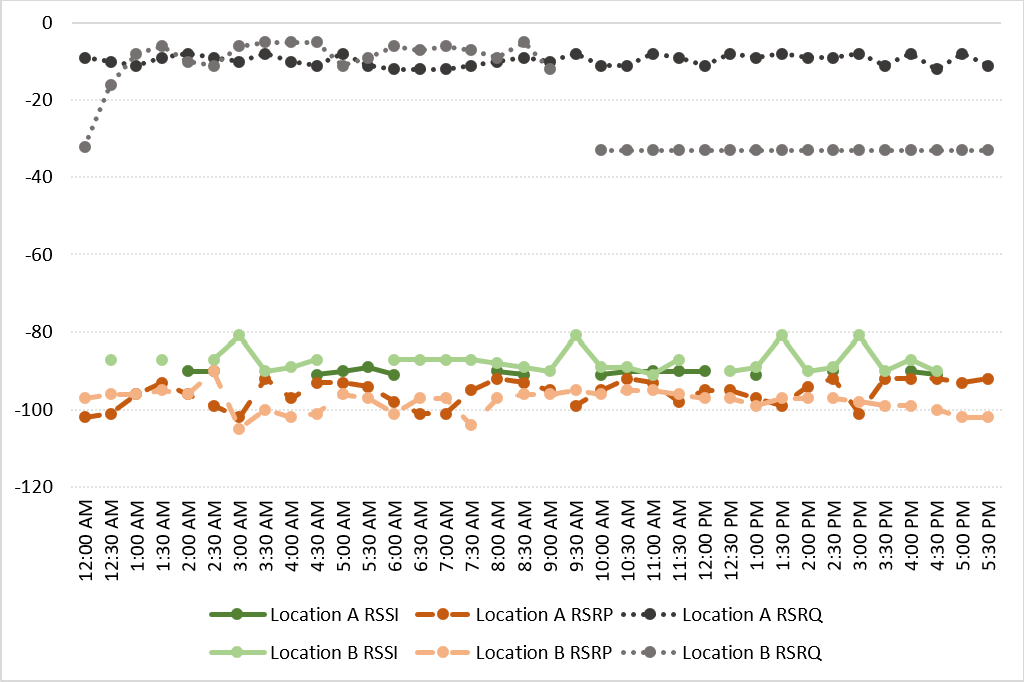
\includegraphics[width=.7\linewidth]{images/tartu/ATartuOut.pdf}  
  \caption{NB-IoT Operator A}
\end{subfigure}
\begin{subfigure}[t]{\linewidth}
  \centering
  % include second image
  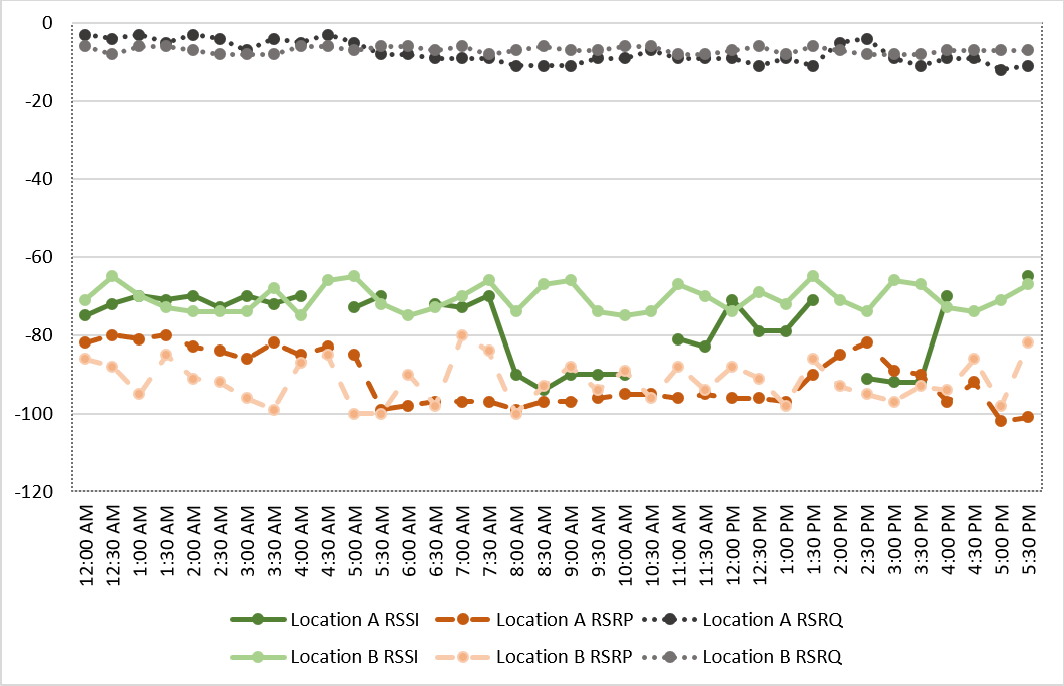
\includegraphics[width=.7\linewidth]{images/tartu/BTartuOut.pdf}  
  \caption{NB-IoT Operator B}
\end{subfigure}

\begin{subfigure}[t]{\linewidth}
  \centering
  % include third image
  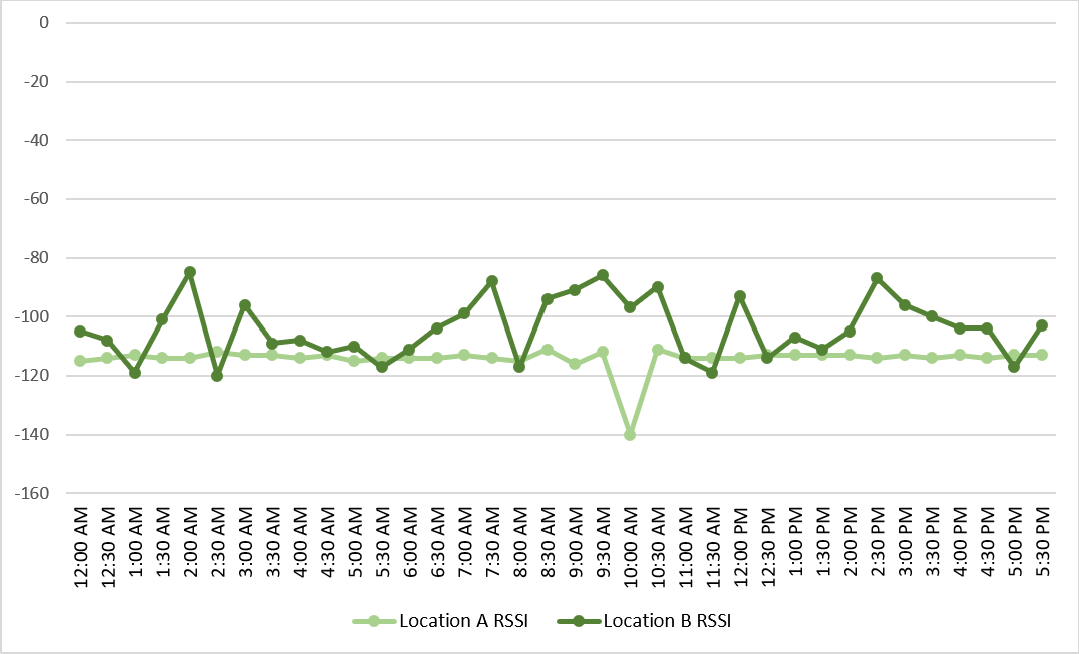
\includegraphics[width=.7\linewidth]{images/tartu/STartuOut.pdf}  
\caption{Sigfox}
 \end{subfigure}
\caption{RF coverage and signal quality: outdoor scenario at University of Tartu}
 \label{RFOutdoor UT}
\end{figure}

%-- Taltech Outdoor figure-- fig 6
 \begin{figure}[h]
\begin{subfigure}[t]{\linewidth}
  \centering
  % include first image
  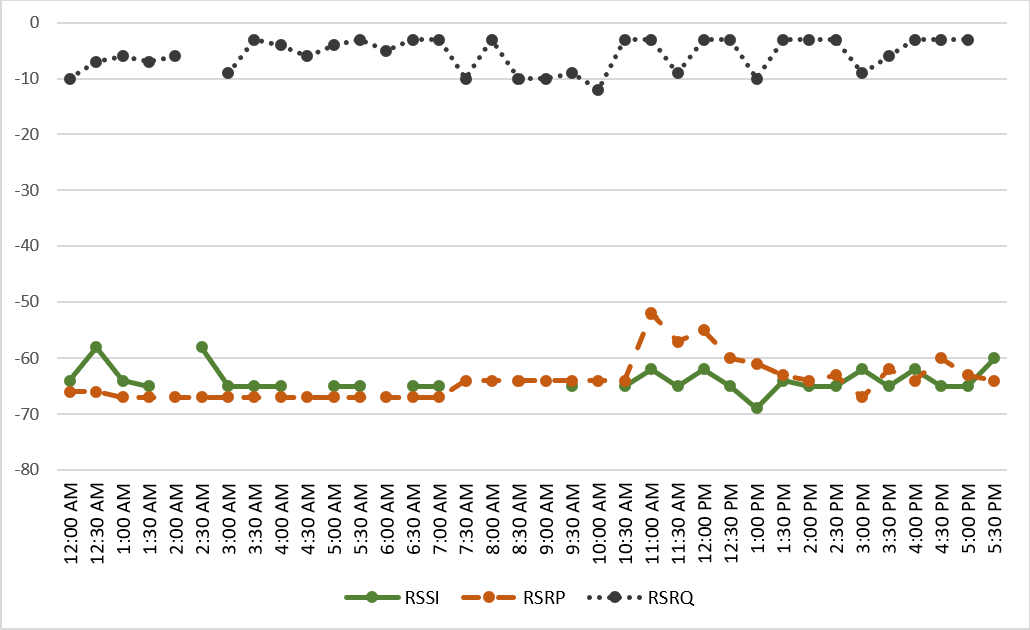
\includegraphics[width=.7\linewidth]{images/tallinn/ATallinnOut.pdf}  
  \caption{NB-IoT Operator A}
\end{subfigure}
\begin{subfigure}[t]{\linewidth}
  \centering
  % include second image
  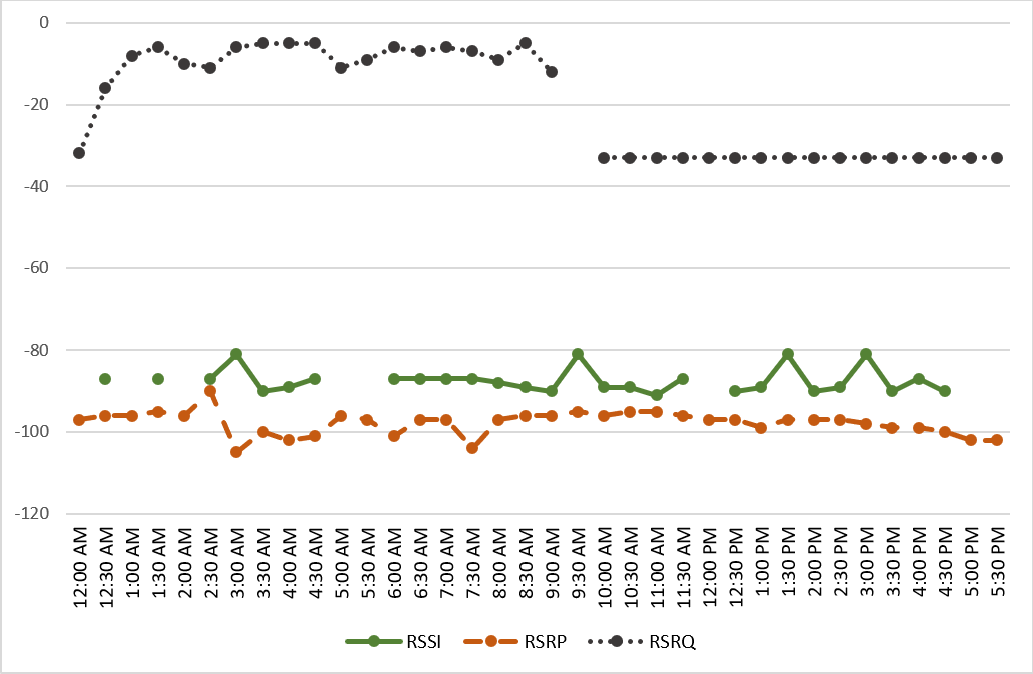
\includegraphics[width=.7\linewidth]{images/tallinn/BTallinnOut.pdf}  
  \caption{NB-IoT Operator B}
  
\end{subfigure}
\begin{subfigure}[t]{\linewidth}
  \centering
  % include third image
  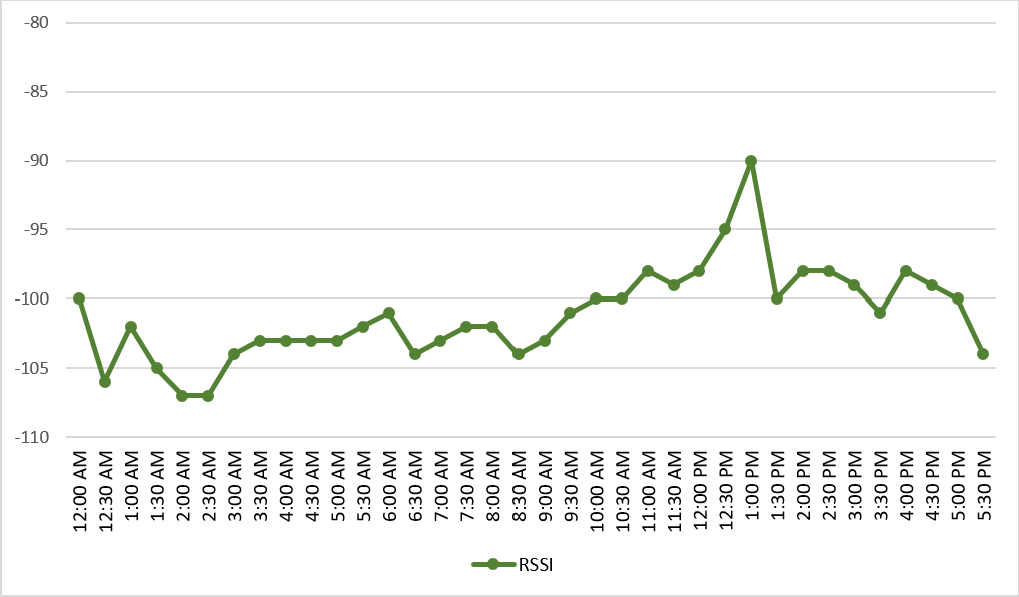
\includegraphics[width=.7\linewidth]{images/tallinn/STallinnOut.pdf}  
\caption{Sigfox}
 \end{subfigure}
\caption{RF coverage and signal quality: outdoor scenario at TalTech}
 \label{RFOutdoor Taltech}
\end{figure}

 Figure \ref{RFOutdoor UT} presents the RF coverage results  in $University\ of\  Tartu$ in Locations A and B shown in Fig. \ref{campus}. In our measurements, it was observed that $operator\ B$ had slightly better outdoor coverage than $operator\ A $ with average RSRP -91.2 dBm compared to -97.4 dBm, as shown in Figure \ref{boxplot}. For RSSI, $operator\ B$ has shown good performance with average RSSI of -77 dBm at location A and -69 dBm RSSI recorded at location B, compared to -90 dBm and -87 dBm, respectively, in case of $operator\ A$. On the other hand, for Sigfox the average RSSI values recorded at Locations A and B were -114 dBm and -103 dBm respectively, which reflects excellent coverage as per \cite{sigfoxRSSI}. For RSRQ, which is defined as quality of received signal \cite{3GPP}, $Operator\ A$ has showed lower RSRQ index at location B compared to $operator\ B$ which shows the weak coverage of $operator\ A$ at this location.\par

In addition to the above, in $Taltech$ Figure \ref{RFOutdoor Taltech}, $operator\ A$ has good coverage with average RSSI value -64 dBM whereas $operator\ B$ has fair coverage with average RSSI value -87 dBm. Similar to RSSI, other parameters RSRP and RSRQ showed similar patterns for $operator\ A$ having median RSRP value -64 dBm compared to -97 dBm in case of $operator\ B$ Figure \ref{boxplot}, and Sigfox on the other hand had good RSSI strength with -101 dBm which reflects excellent coverage as per Table \ref{sigfoxRSSI}.\par
It is important to highlight NB-IoT and Sigfox both had 0\% packet loss for the outdoor scenario.


%-- Tartu Indoor figure
 \begin{figure}[t]
\begin{subfigure}[t]{\linewidth}
  \centering
  % include first image
  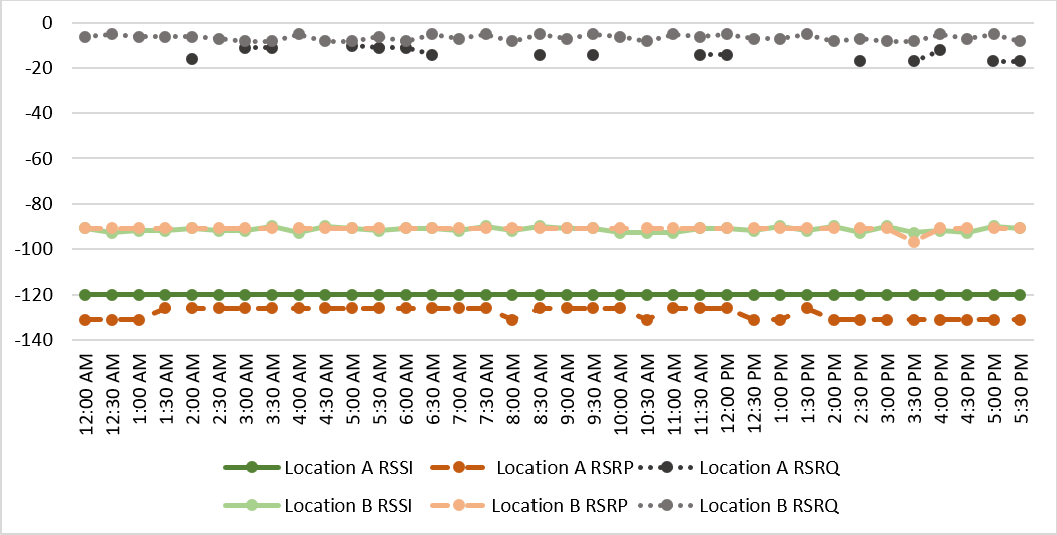
\includegraphics[width=.7\linewidth]{images/tartu/ATartuIndoor.pdf}  
  \caption{NB-IoT Operator A}
\end{subfigure}
\begin{subfigure}[t]{\linewidth}
  \centering
  % include second image
  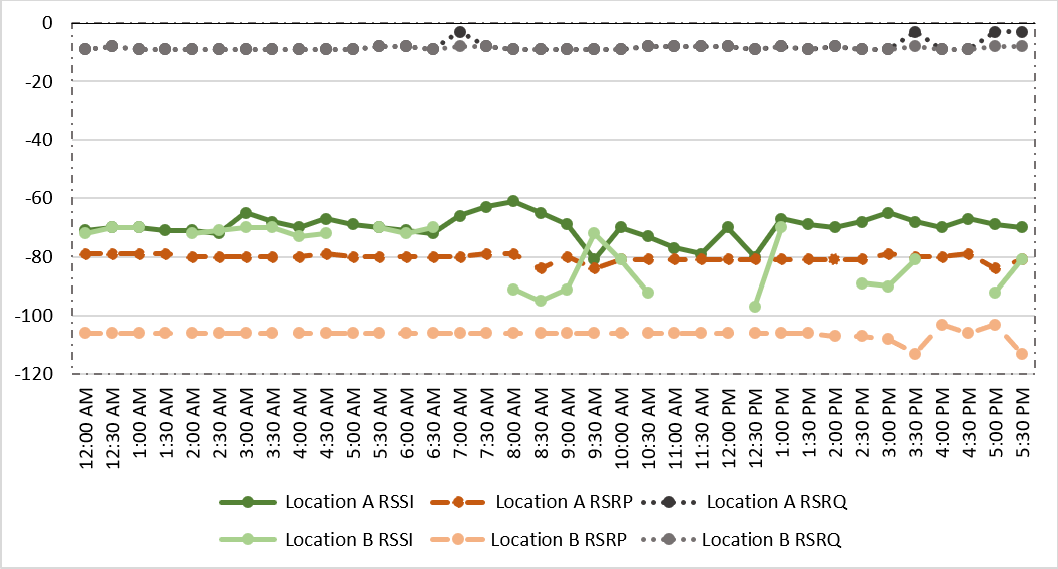
\includegraphics[width=.7\linewidth]{images/tartu/BTartuIndoor.pdf}  
  \caption{NB-IoT Operator B}
  
\end{subfigure}
\begin{subfigure}[t]{\linewidth}
  \centering
  % include third image
  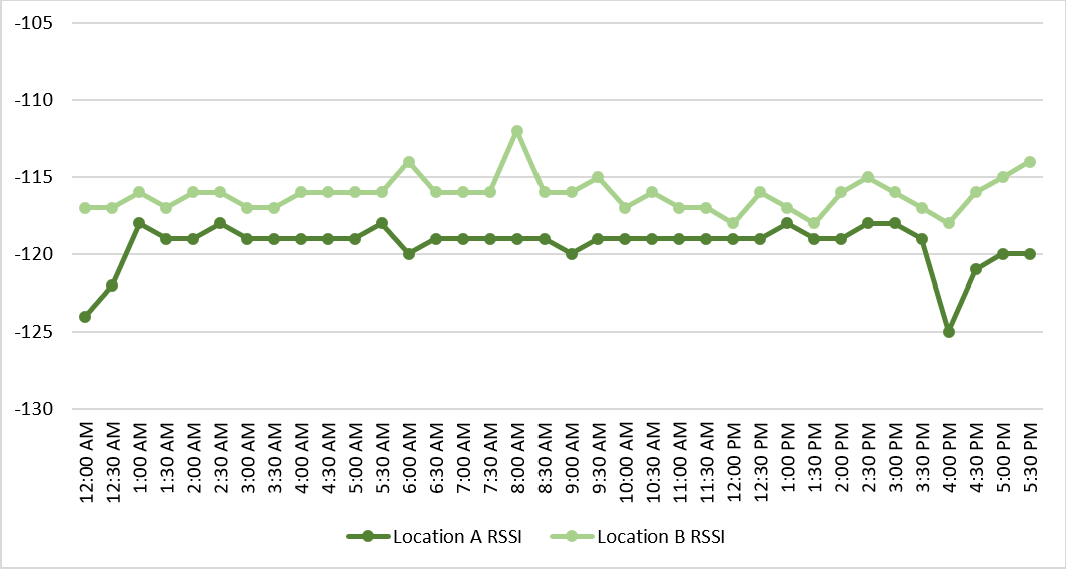
\includegraphics[width=.7\linewidth]{images/tartu/STartuIndoor.pdf}  
\caption{Sigfox}
 \end{subfigure}
\caption{RF coverage and signal quality: indoor scenario at University of Tartu}
 \label{RFIndoor Tartu}
\end{figure}

%-- Tallinn Indoor figure
 \begin{figure}[t]
\begin{subfigure}[t]{\linewidth}
  \centering
  % include first image
  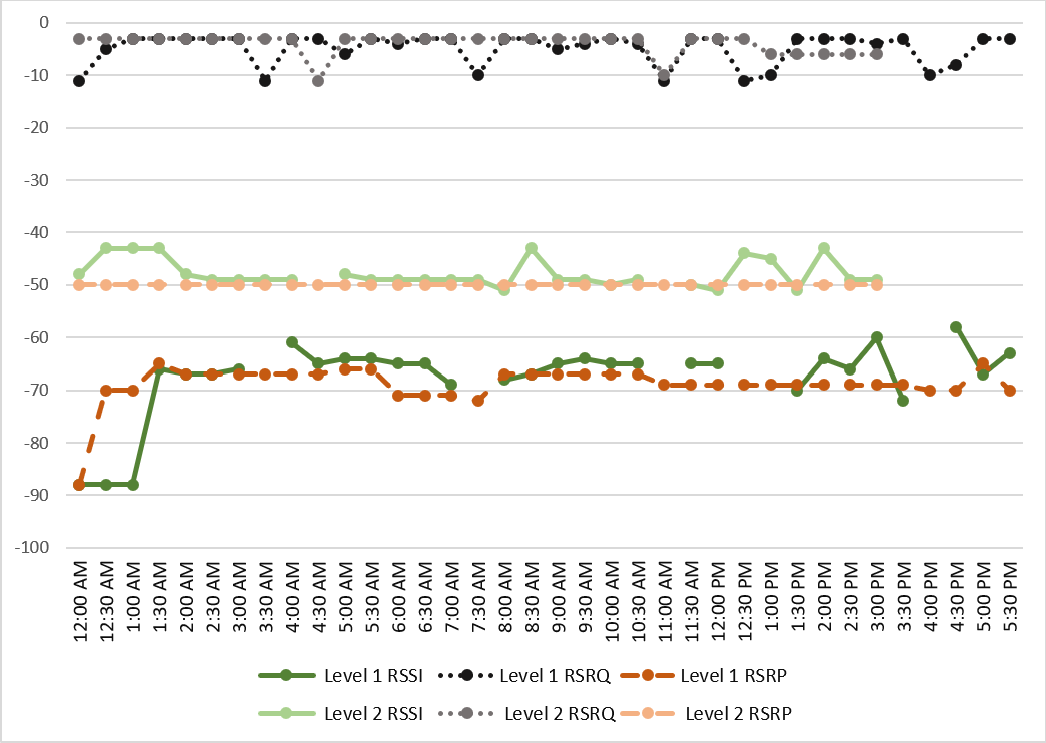
\includegraphics[width=.7\linewidth]{images/tallinn/ATallinnIndoor.pdf}  
  \caption{NB-IoT Operator A}
\end{subfigure}
\begin{subfigure}[t]{\linewidth}
  \centering
  % include second image
  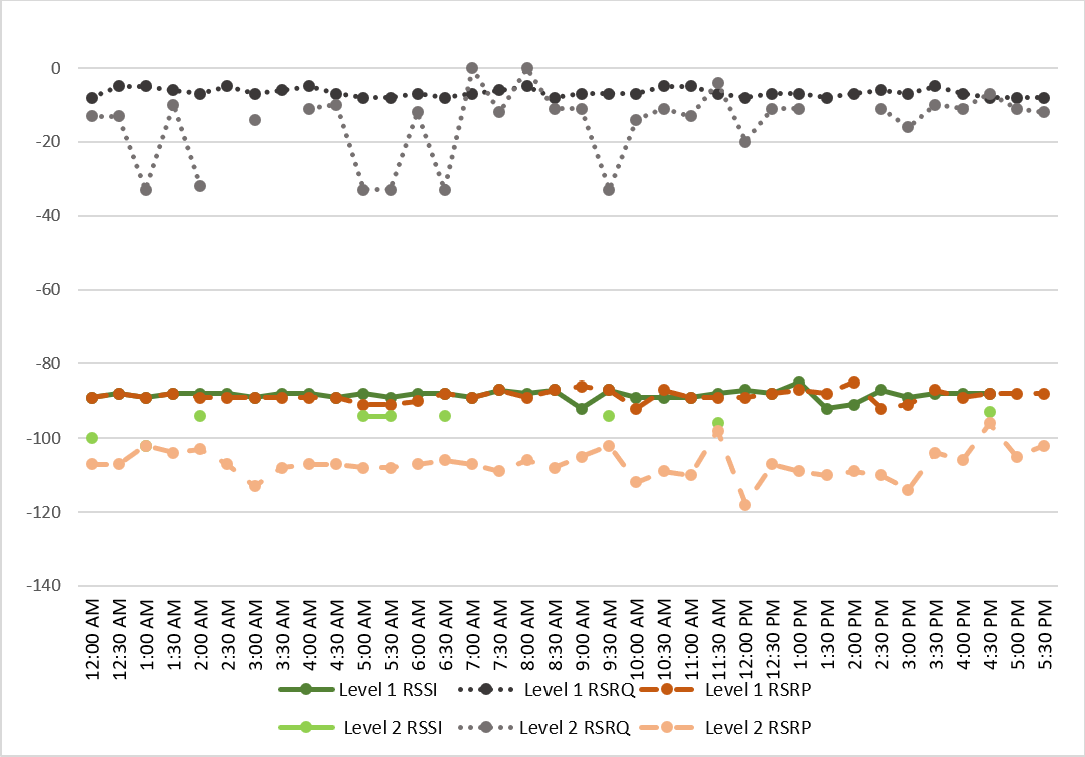
\includegraphics[width=.7\linewidth]{images/tallinn/BTallinnIndoor.pdf}  
  \caption{NB-IoT Operator B}
  
\end{subfigure}
\begin{subfigure}[t]{\linewidth}
  \centering
  % include third image
  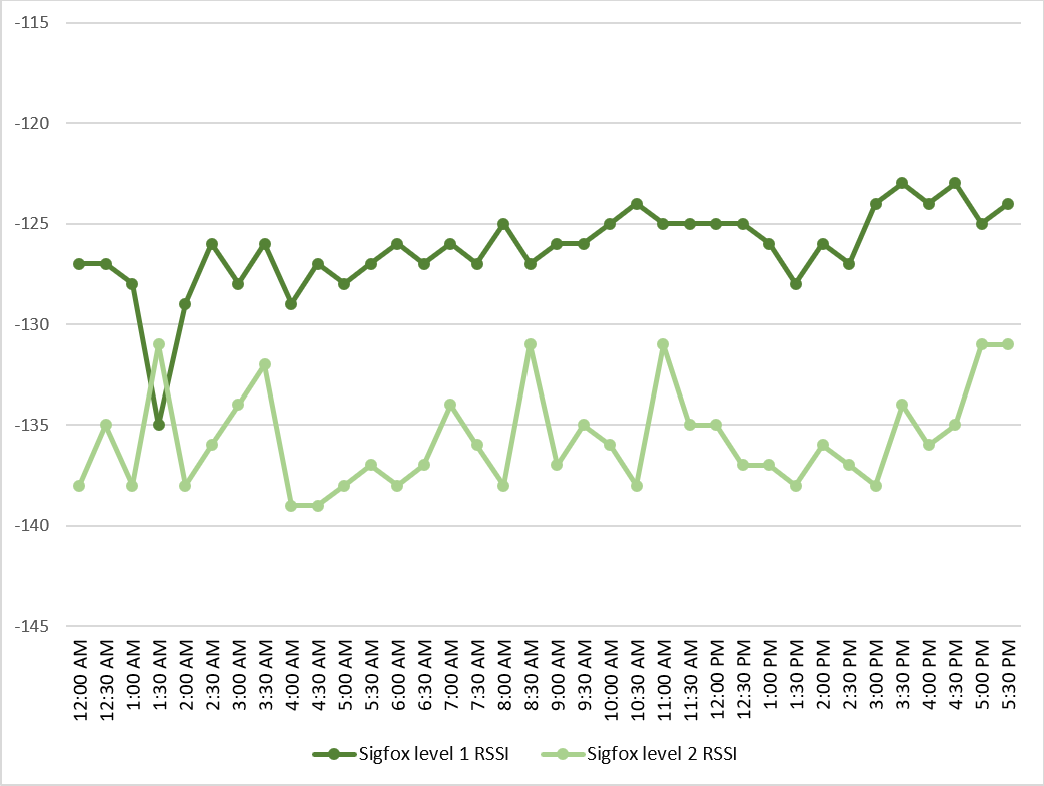
\includegraphics[width=.7\linewidth]{images/tallinn/STallinnIndoor.pdf}  
\caption{Sigfox}
 \end{subfigure}
\caption{RF coverage and signal quality: indoor scenario at in TalTech}
 \label{RFIndoor Tallinn}
\end{figure}

\subsection{Indoor}\label{Indoor}

Figure \ref{RFIndoor Tartu} illustrates the RSSI, RSRP and RSRQ values in indoor scenarios in both campuses. In our measurement, at $University\ of\ Tartu$ Location A, for NB-IoT $operator\ A$, our nodes did not measured any RSSI strength, which is result of RSRP above the threshold value.The average RSRP and RSRQ index measured were -128 dBm and -14 dB, which reflects poor coverage as per Table \ref{nbiotRSRP}. However, interestingly, even with weaker coverage strength there were no packet loss which shows NB-IoT reliability and robustness which is due to the fact that a packet can be re-transmitted (up to 128 repetitions in uplink), which increases the success probability at the price of energy consumption.
It was also observed in Location A that with the increase in human occupancy in the building, which is directly proportional to active mobile users, there were fluctuations in the RSSI in both NB-IoT operators; however, the same was not observed with Sigfox, which shows that Sigfox is unaffected by neighboring LTE interference and noises which is due to its ultra narrow band modulation.

Furthermore, at TalTech campus, see Figure \ref{RFIndoor Tallinn}, it was observed that NB-IoT $operator\ A$ had better coverage compared to $Operator\ B$. During the measurement cycle, the average RSRP calculated  was -68 dBm for $Operator\ A$ with respect -88 dBm at level 1 for $operator\ B$. For the same settings at level 2 the average RSRP value for $operator\ B$ increased to -107 dBM compared to -54 dBm in case of $operator\ A$. 

For both campuses in indoor scenario, we have observed few packet losses in Sigfox compared to NB-IoT, which shows that even with weaker signal strength NB-IoT is reliable and resilient.\par


\subsection{Deep Indoor}
Figure \ref{RFDeepIndoorTartu} and Figure \ref{RFDeepIndoorTallinn} presents the RF coverage of NB-IoT and Sigfox in deep-indoor. It is interesting to note that NB-IoT $operator\ A$ had NB outage in $University\ of\ Tartu$ location A. Therefore, it has been assigned value 0 for all corresponding RF parameters. However, on the other hand $operator\ B$ had maximum packet loss of 61\%, followed by Sigfox for same location that had 9\% packet loss. The average RSRP observed, see Figure \ref{boxplot}, at this site was -133 dBm for $operator\ B$ which quantifies to\ poor coverage. In addition to the above, at location B of $University\ of\ Tartu$ there were 33\% of packet loss in case of NB-IoT $Operator\ B$, followed by 0\% packet loss in case of $operator\  A$, which confirms that $operator\ B$ has weaker deep indoor coverage penetration at this location.This observation also confirms, NB-IoT performances are affected by building structure and material used.

%-- Tartu DeepIndoor figure
 \begin{figure}[t]
\begin{subfigure}[t]{\linewidth}
  \centering
  % include first image
  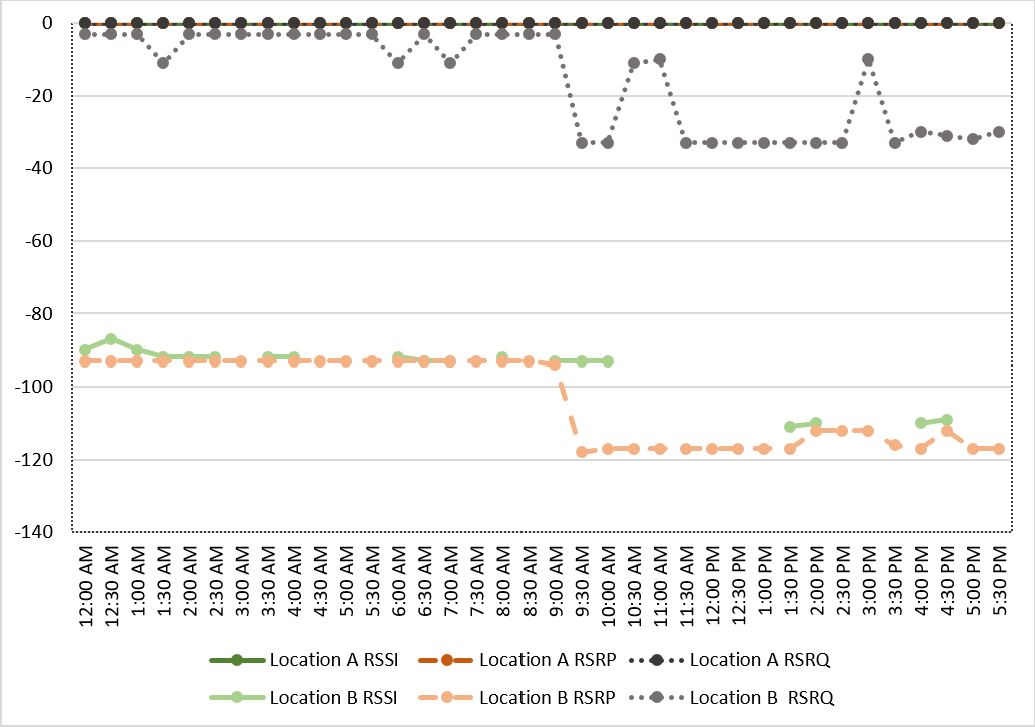
\includegraphics[width=.7\linewidth]{images/tartu/ATartuDeepIndoor.pdf}  
  \caption{NB-IoT Operator A}
\end{subfigure}
\begin{subfigure}[t]{\linewidth}
  \centering
  % include second image
  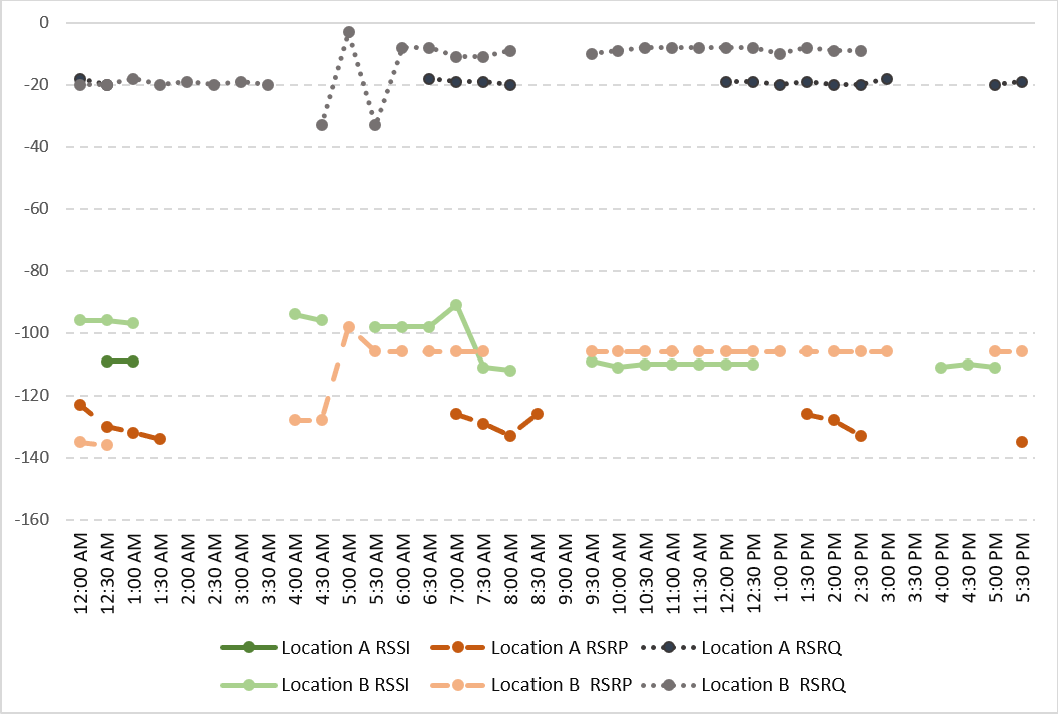
\includegraphics[width=.7\linewidth]{images/tartu/BTartuDeepIndoor.pdf}  
  \caption{NB-IoT Operator B}
  
\end{subfigure}
\begin{subfigure}[t]{\linewidth}
  \centering
  % include third image
  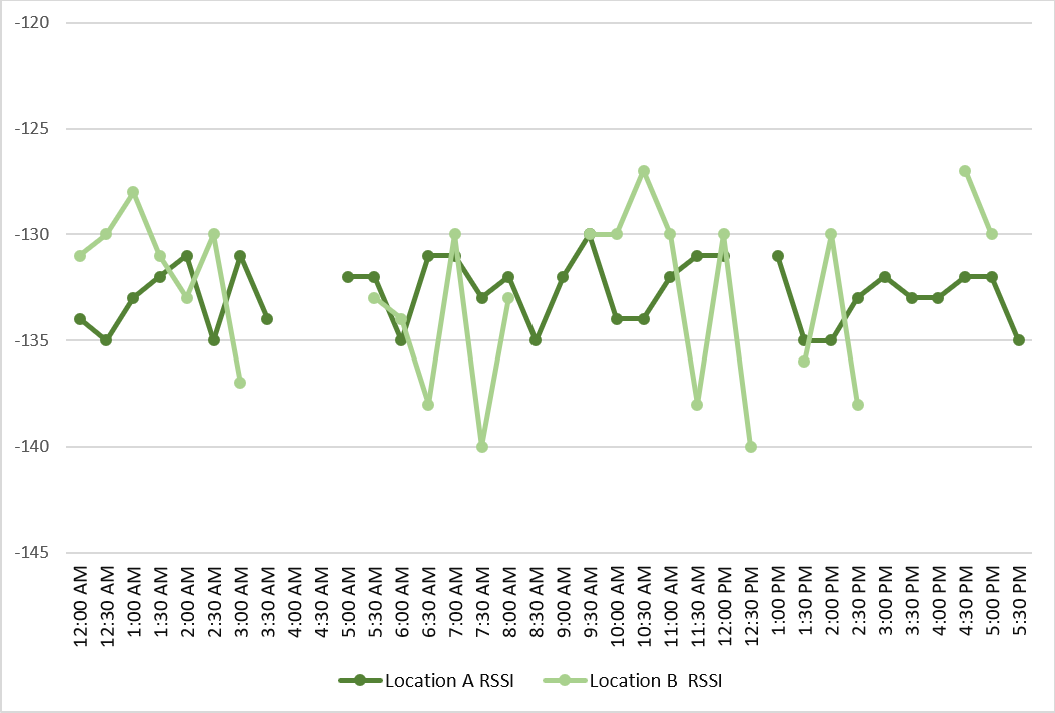
\includegraphics[width=.7\linewidth]{images/tartu/STartuDeepIndoor.pdf}  
\caption{Sigfox}
 \end{subfigure}
\caption{RF coverage and signal quality: deep indoor scenario in University of Tartu}
 \label{RFDeepIndoorTartu}
\end{figure}



%-- Tallinn DeepIndoor figure
 \begin{figure}[t]
\begin{subfigure}[t]{\linewidth}
  \centering
  % include first image
  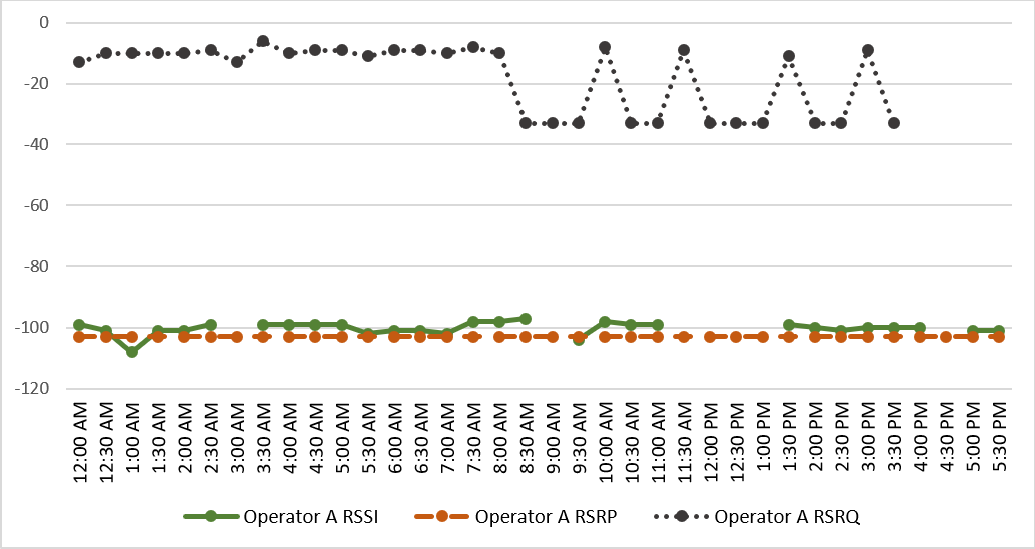
\includegraphics[width=.7\linewidth]{images/tallinn/ATallinnDeepIndoor.pdf}  
  \caption{NB-IoT Operator A}
\end{subfigure}
\begin{subfigure}[t]{\linewidth}
  \centering
  % include second image
  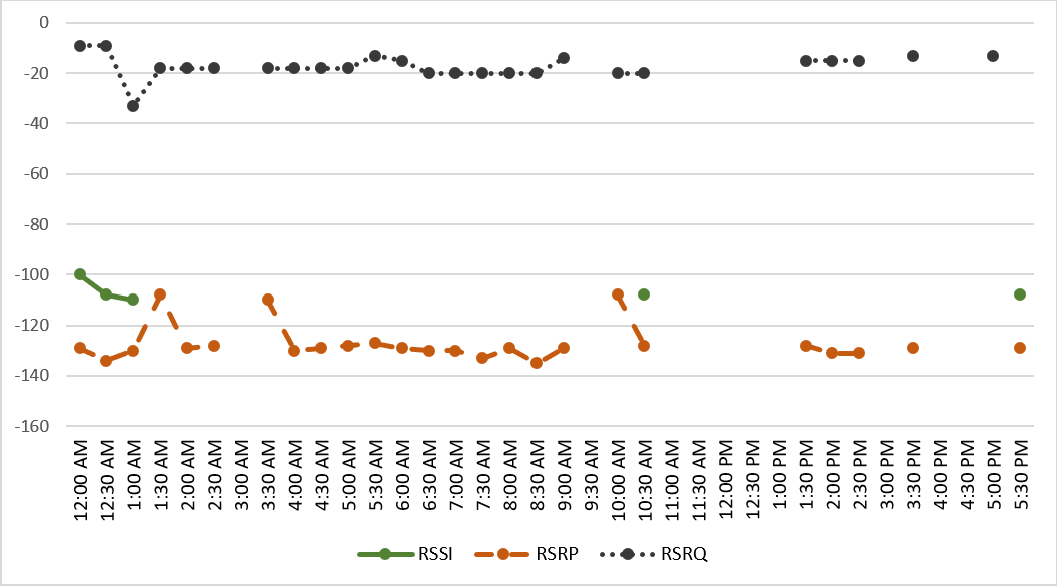
\includegraphics[width=.7\linewidth]{images/tallinn/BTallinnDeepIndoor.pdf}  
  \caption{NB-IoT Operator B}
  
\end{subfigure}
\begin{subfigure}[t]{\linewidth}
  \centering
  % include third image
  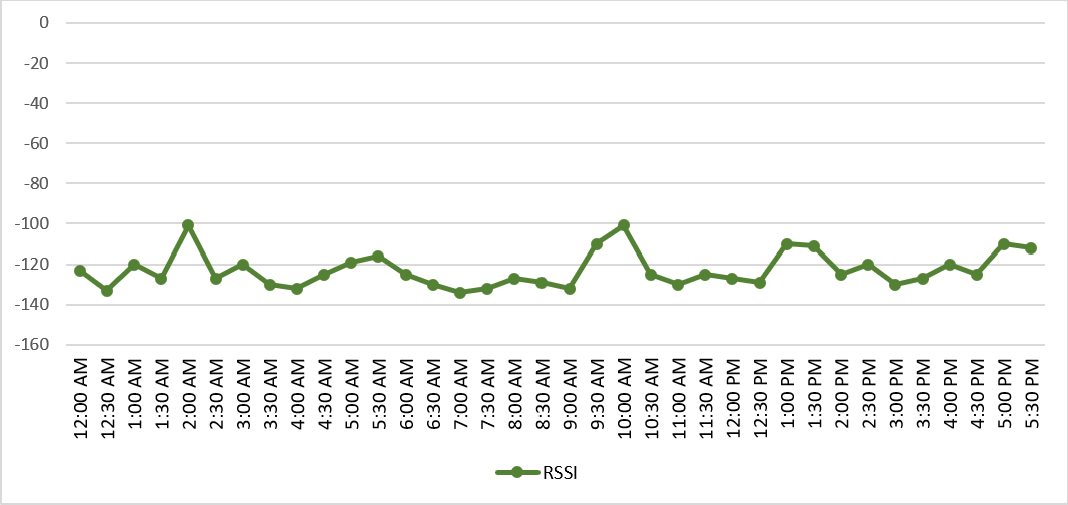
\includegraphics[width=.7\linewidth]{images/tallinn/STallinnDeepIndoor.pdf}  
\caption{Sigfox}
 \end{subfigure}
\caption{RF coverage and signal quality: deep indoor scenario in TalTech}
 \label{RFDeepIndoorTallinn}
\end{figure}


Furthermore, the same outage and high packet loss was not observed in TalTech campus for NB-IoT which shows both operators $operator\ A$ and $operator\ B$ have dense narrow band network in that area at the time of writing this paper.


%-- RSRP Boxplot figure
 \begin{figure}[ht!]
\begin{subfigure}[t]{\linewidth}
  \centering
  % include first image
  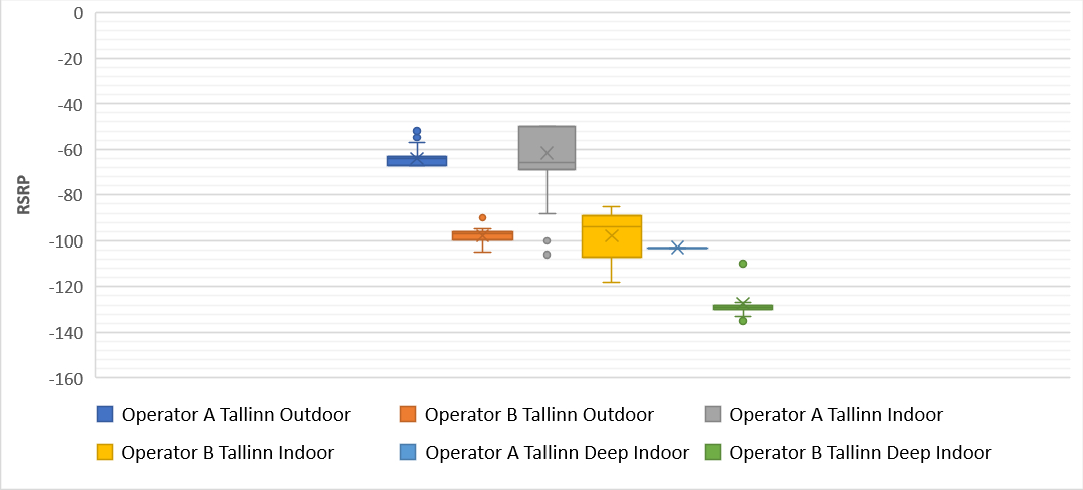
\includegraphics[width=.7\linewidth]{images/TallinnRSRPboxplot.pdf}  
  \caption{TalTech campus, Tallinn}
\end{subfigure}
\begin{subfigure}[t]{\linewidth}
  \centering
  % include second image
  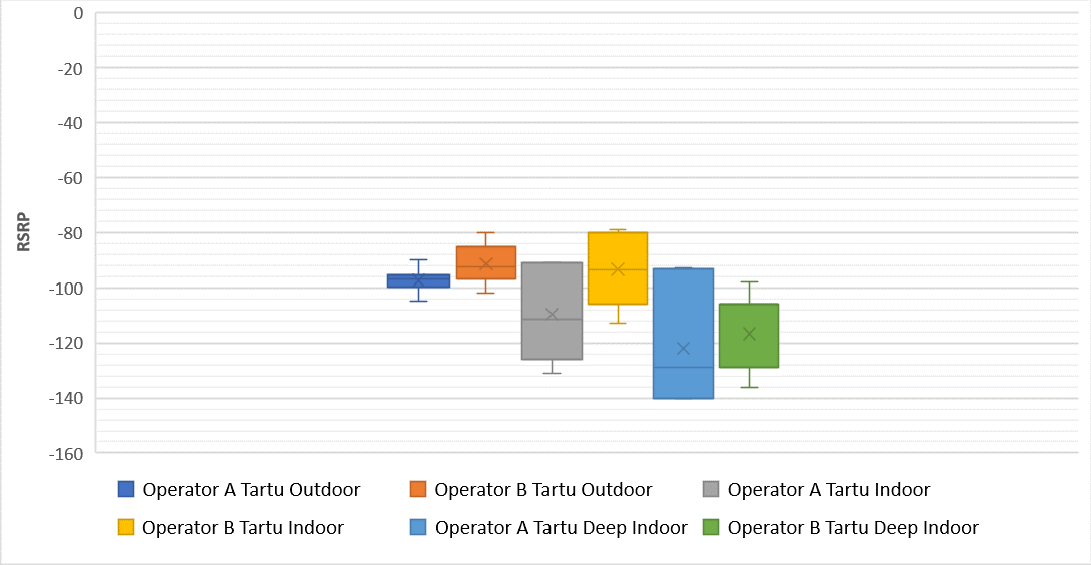
\includegraphics[width=.7\linewidth]{images/TartuRSRPboxplot.pdf}  
  \caption{University of Tartu campus, Tartu}
  
\end{subfigure}
\caption{NB-IoT RSRP distribution in Tallinn and Tartu}
 \label{boxplot}
\end{figure}

\section{CONCLUSION} \label{conclusion}
In this paper we provided an evaluation of real-time coverage of NB-IoT and Sigfox in two university campuses in the two main cities of Estonia (Tartu and Tallinn).These results provides a comprehensive overview of coverage recorded in different scenarios and can be further used by operators as a reference point. The coverage and signal quality results showed promising performance for Outdoor and Indoor scenarios. However, for NB-IoT Deep Indoor scenario the results were better in TalTech as compared to University of Tartu. Sigfox, on the other hand, achieved a good coverage in both campuses in Outdoor, Indoor and Deep-Indoor scenarios with very minimum packet losses (pack losses which were observed in Indoor and Deep-Indoor with NB-IoT).\par
In future contribution, we would extend our investigation with different radio modems, environment conditions and also plan to analyse the data rate and energy efficiency of LPWAN technologies.

\section{ACKNOWLEDGMENT}\label{ack}
This project has received funding partly from European Union’s Horizon 2020 Research and Innovation Program under Grant 668995 and European Union Regional Development Fund in the framework of the Tallinn University of Technology Development Program 2016–2022 and Archimedes Foundation Smart specialisation scholarship. This work has also been conducted in the framework of the Estonian Centre of Excellence in ICT Research (Excite). We are also thankful to Connected Baltics OÜ, Telia Eesti AS and Elisa Eesti AS for providing us resources to conduct this research.

\bibliographystyle{IEEEtran}

\bibliography{references}

\end{document}